\documentclass[12pt]{article}

\PassOptionsToPackage{english}{babel}
\usepackage{pablo}
\selectlanguage{english}

\usepackage{multicol}

\usepackage[a4paper,margin=0.9cm]{geometry}

\usepackage{pablo-listings}

\usetikzlibrary{decorations.fractals}

\pagestyle{empty}

\begin{document}

\begin{center}
  Algorithmic

  {\large
    \textsc{Turtle}
  }

  ------------------
\end{center}

\section{First steps with IDLE}

\begin{multicols}{2}
\begin{enumerate}
  \item Launch IDLE.
  \item Open a new file : \texttt{File > New Window}.
  \item Copy the program printed on the right in the new window.
  \item Run this program : \texttt{Run > Run module}.
  \item What does this program do ?
\end{enumerate}

\columnbreak

\begin{lstlisting}[language=python,frame=single]
from turtle import *

forward(200)
left(90)
forward(100)
left(90)
forward(200)
left(90)
forward(100)

mainloop()
\end{lstlisting}

\end{multicols}

\section{Square}

\begin{enumerate}
  \item Write a program that draws a square.
  \item Write a program that draws a regular pentagon.
\end{enumerate}

\section{Loops}

\begin{multicols}{2}
  The program used to draw the latter figure was repetitive: the same lines were copied five times. Instead of doing this, lets just tell the computer to run a few lines five times.

\begin{enumerate}
  \item Copy and run the program displayed on the right.
  \item Using the same method, draw a regular polygon with 10 sides.
\end{enumerate}

\columnbreak

\begin{lstlisting}[language=python,frame=single]
from turtle import *

for i in range(4):
    forward(100)
    left(90)

mainloop()
\end{lstlisting}
\end{multicols}

\begin{enumerate}
  \setcounter{enumi}{2}
  \item Draw the following figures.
\end{enumerate}

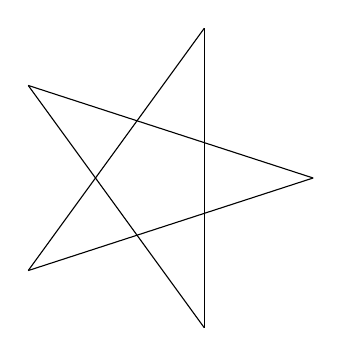
\begin{tikzpicture}[scale=2]
  \foreach \i in {1,...,5} {
    \draw ({\i *360/5}:1) -- ({(\i +2)*360/5}:1);
  }
\end{tikzpicture}
\hspace{\stretch{1}}
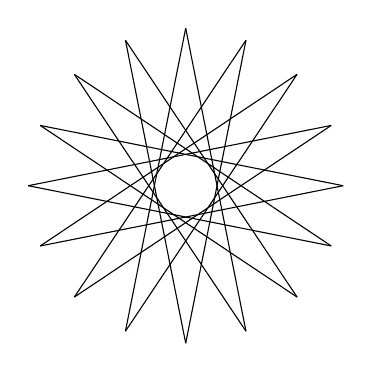
\begin{tikzpicture}[scale=2]
  \foreach \i in {1,...,16} {
    \draw ({\i *360/16}:1) -- ({(\i +7)*360/16}:1);
  }
\end{tikzpicture}
\hspace{\stretch{1}}
\begin{tikzpicture}[scale=1.5]
  \foreach \i in {1,...,6} {
    \begin{scope}[shift={(-1.5,5.5)},rotate={\i*360/6}]
      \draw (-0.5,-0.86602) -- (1.5,-0.86602) -- (1.5, -1.86602) -- (0.5,-1.86602) -- (0.5,-0.86602);
    \end{scope}
  }
\end{tikzpicture}

\section{Assignment}

~

\begin{multicols}{2}
  Now, we want to draw the following figure.

\begin{center}
  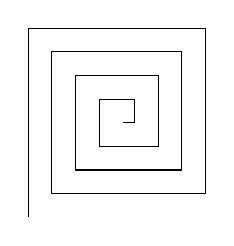
\begin{tikzpicture}[scale=0.15]
    \draw (0,0) -- ++(1,0) -- ++(0,2) -- ++(-3,0) -- ++(0,-4)
    -- ++(5,0) -- ++(0,6) -- ++(-7,0) -- ++(0,-8)
    -- ++(9,0) -- ++(0,10) -- ++(-11,0) -- ++(0,-12)
    -- ++(13,0) -- ++(0,14) -- ++(-15,0) -- ++(0,-16);
  \end{tikzpicture}
\end{center}

To do so, we are using a variable \texttt{length} representing the current line segment size. This variable will be incremented as the length of the segments raises.

A program implementing this is given on the right.

\columnbreak

\begin{lstlisting}[language=python,frame=single]
from turtle import *

length = 0

while length < 200:
    forward(length)
    left(90)
    length = length + 10

mainloop()
\end{lstlisting}

\end{multicols}

Draw the following figure.
\begin{center}
  \begin{tikzpicture}[scale=0.5]
  \foreach \i in {1,...,5} {
    \draw ({(0.5*\i*\i)-0.5*\i},0) -- ++ (\i, 0) -- ++ (0,\i) -- ++(-\i, 0) -- cycle;
  }
  \end{tikzpicture}
\end{center}

\section{Drunkard walk}

\begin{multicols}{2}

  ~

  \begin{enumerate}
    \item Copy and run the program on the right.
    \item What does function \texttt{randint} do ?
    \item Consider the following problem: a drunk turtle tries to walk across
      a bridge without any safety barrier. Each step is done, at random,
      forward, on the left, or on the right. Unfortunately, the bridge in
      only four steps wide.

      Enhance the program so that it stops as soon as the turtle falls off the bridge.
  \end{enumerate}

  ~

  \columnbreak

\begin{lstlisting}[language=python,frame=single]
from turtle import *
from random import randint

while True:
    alea = randint(-1,1)
    if alea == 0:
        forward(10)
    elif alea == -1:
        left(90)
        forward(10)
        right(90)
    else:
        right(90)
        forward(10)
        left(90)


mainloop()
\end{lstlisting}
\end{multicols}

\section{Further works}

\begin{multicols}{2}
  \noindent Draw the \emph{Koch snowflake} (right figure).

  \noindent You will have to use functions (you can omit them, but it is more complicated). You can look for help on the Internet.

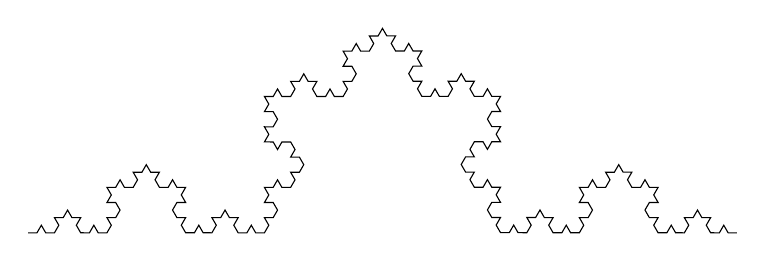
\begin{tikzpicture}[decoration=Koch snowflake,scale=3]
  \draw decorate{ decorate{ decorate{ decorate{ (0,0) -- (3,0) }}}};
\end{tikzpicture}
\end{multicols}

\end{document}
